%
% loesung.tex -- Beispiel-File für die Beschreibung der Loesung
%
% (c) 2020 Prof Dr Andreas Müller, Hochschule Rapperswil
%
\section{Lösung
\label{fem:section:loesung}}
\rhead{Lösung}
Wie im vorherigen Kapitel erwähnt sind Herausforderungen bzw. Ansprüche an die Ansatzfunktionen zu beachten. Nun stellt sich die Frage, wie die Ansatzfunktion gewählt werden müssen, so das entlang eines Randes nur \frqq Knicke \flqq entstehen und keine Sprünge. Und wie ist gewährleistet das in der gleichen Stützstelle alle Elemente den gleichen Wert haben?  Als Lösungs bietet sich ein lineare Funktion an. Für das Dreieck  ist es der Term $u(x) = c_1 + c_2x + c_3y$ an. Diese Zusammensetzung ergibt sich, da der lineare Ansatz durch die Funktionswerte in den Ecken des Dreiecks bestimmt wird. In anderen Worten ausgedrückt sind die Funktionswerte in den Ecken des Teilgebiets, hier im Dreieck, die Unbekannten, die bestimmt werden müssen. Wie diese Koeffizienten in einer Matrix bestimmt werden ist in \ref{fem:section:GL} aufgezeigt.

%\begin{figure}[h!]
%	\centering
%	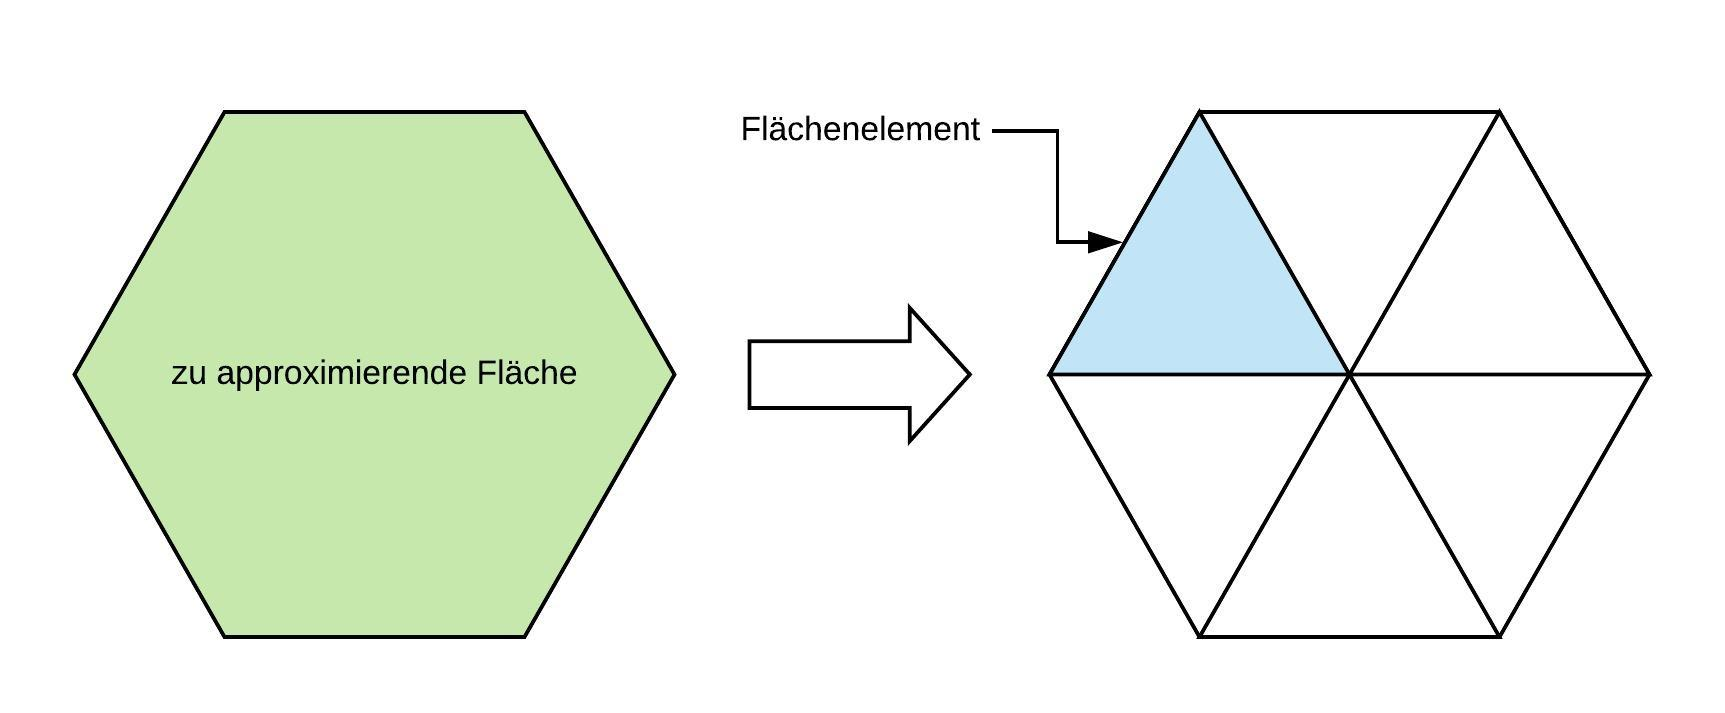
\includegraphics[scale=0.8]{papers/fem/Images/Approx.jpeg}
%	\caption{Flächen- Approximation mit Dreiecks- Flächenelemente}
%	\label{fem:Approx}
%\end{figure}
Nochmals zur Verdeutlichung warum ein linearer Ansatzfunktion verwendet wird:
\begin{itemize}
	\item eine einfache Formel gibt es nur auf einem kleinen Teilgebiet
	\item in dem Teilgebiet ist die Integral- Formel sehr einfach zu berechnen wie z.B. eine lineare Funktion die durch Koeffizienten bestimmt wird.
\end{itemize}
%ls Standardverfahren in der Ebene haben sich Flächenelement wie Dreiecken oder Parallelogramme bewährt. Die Wahl der  der Flächen- bzw. Gebiet- Elementen sollte so erfolgen, dass diese die zu approximierende Fläche möglichst gut nachbildet bzw. approxmimiert wird.
Um möglichst einfach darzustellen, wie das Verfahren der Finiten Elemente vonstatten geht, wurde auf eine einfache Approximation mit Einheitsdreiecken und einem linearen Ansatz gewählt. 

\subsection{Vorbereitung
\label{fem:section:loesungTrans}}

Damit die Integration über das gewählte Teilgebiet einfacher fällt, wird als Vorbereitung im entsprechenden Fall das gewählte Gebiet in ein Einheitsdreieck oder in ein Einheitsparallelogramm transformiert. So können alle Gebiete gleich behandelt und berechnet werden. \\
Das allgemeine Dreieck in allgemeiner Lage mit den Eckpunkten $P_1(x_1, y_1$), $ P_2(x_2, y_2)$ und $P_3(x_3,y_3)$ kann mit Hilfe der linearen Transformation
\begin{equation}
	\begin{split}
		x = x_1 + (x_2 - x_1)\xi + (x_3 - x_1)\eta \\
		y = y_1 + (y_2 - y_1)\xi + (y_3 - y_1)\eta
		\label{fem:linTransformation}
	\end{split}
\end{equation}
in das einfachere Gebiet nämlich das gleichschenklig rechtwinklige Einheitsdreieck mit Kathetenlänge 1 überführt werden wie in der Abbildung \ref{fig:TransformationEinheitsdreieckBild} dargestellt ist.

\begin{figure}[h!]
	\centering
	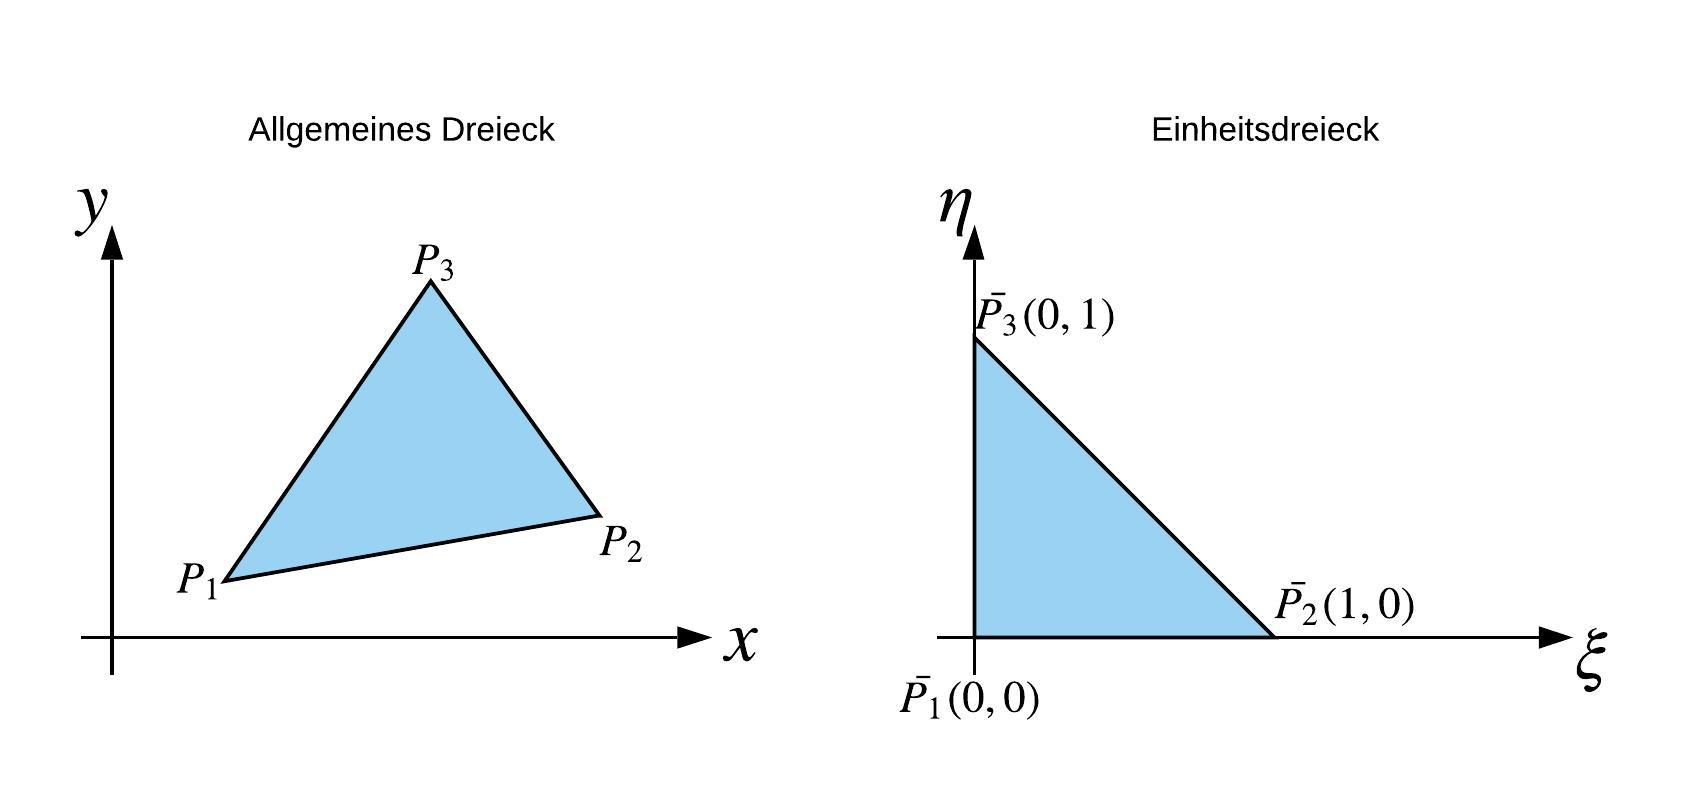
\includegraphics[scale=0.8]{papers/fem/Images/Dreiecke.jpeg}
	\caption{Transformation in ein Einheitsdreieck}
	\label{fig:TransformationEinheitsdreieckBild}
\end{figure}
Die Variablen \xi und \eta werden die neuen Integrationsvariablen.
\begin{equation}
			dy \, dy = \det(J) \, d\xi \, d\eta
			\label{fem:newTransformation}
\end{equation}
Damit die Berechnung korekt ist, muss noch die Determinante der Jacobi Matrix dazu noch multipliziert werden.
\begin{equation}
J % 
=
\begin{bmatrix}
    \frac{\partial x}{\partial \xi} &  \frac{\partial x}{\partial \eta}     \\
   \frac{\partial y}{\partial \xi}  &  \frac{\partial y}{\partial \eta}     
\end{bmatrix}
= 
\begin{bmatrix}
    x_2 - x_1  &  x_3 -x_1      \\
    y_2 - y_1  &  y_3 - y_1      
\end{bmatrix} 
	\label{fem:Jocobi}
\end{equation}
Die Jacobi Matrix \ref{fem:Jocobi} besteht aus den partiellen Ableitungen aus \ref{fem:linTransformation}.  
\begin{equation}
	\det(J) = x_1 \cdot y_2 - 2 \cdot x_1 \cdot y_1 + x_2 \cdot y_1 + x_1\cdot y_3 + x_3 \cdot y_1 - x_2 \cdot y_3 - x_3 \cdot y_2
	\label{fem:JocobiDetBerechnet}
\end{equation}
Determinante von \ref{fem:Jocobi} ist \eqref{fem:JocobiDetBerechnet}. Die Jacobi- Determinante entspricht der doppelten Fläche des Dreiecks. Die partiellen Ableitungen werden gemäss der Kettenregel zu 
%\begin{equation}
%			\begin{aligned}
%			u_x = u_{\xi} \xi_x + u_{\eta} \eta_x \\
%			u_y = u_{\xi} \xi_y + u_{\eta} \eta_y 
% 			\end{aligned}
%			\label{fem:newKoordinate}
%\end{equation}
\begin{equation}
\begin{split}
	\frac{\partial u}{\partial x} = \frac{\partial u}{\partial \xi} \, \frac{\partial \xi}{\partial x} + \frac{\partial u}{\partial \eta} \, \frac{\partial \eta}{\partial x} \\
	\frac{\partial u}{\partial y} = \frac{\partial u}{\partial \xi} \, \frac{\partial \xi}{\partial y} + \frac{\partial u}{\partial \eta} \, \frac{\partial \eta}{\partial y}
	\end{split}
\end{equation}
Auf Grund der linearen Transformation \eqref{fem:linTransformation} ergeben sich nach der partieller Differentiation der beiden Beziehungen nach $x$ zunächst

\begin{equation}
			\begin{aligned}
			1  = (x_2 -x_1) \, \frac{\partial \xi}{\partial x} + (x_3 -x_1) \, \frac{\partial \eta}{\partial x} \\
			0 = (y_2 -y_1) \, \frac{\partial \xi}{\partial x} + (y_3 -y_1) \, frac{\partial \eta}{\partial x} \\
			 \end{aligned}
\end{equation}
Nach Auflösung  der beiden Gleichungen nach $\frac{\partial \xi}{\partial x}$ und $\frac{\partial \eta}{\partial x}$ ergibt sich
\begin{equation}
			\frac{\partial \xi}{\partial x} = \frac{y_3 - y_1}{J} \quad \frac{\partial \eta}{\partial x} = -\frac{y_2 - y_1}{J}
\end{equation}
Analog nach der partiellen Ableitung nach $y$ erhält man

\begin{equation}
			\frac{\partial \xi}{\partial y} = \frac{x_3 - x_1}{J} \quad \frac{\partial \eta}{\partial y} = -\frac{x_2 - x_1}{J}
\end{equation}
Somit vereinfacht sich die Integration über das Einheitsdreieck 
\begin{equation}
			\int_{\triangle} u \quad dy \, dx = \int_0^1 \int_0^{1 - \xi} \, u \det (J) \, d \eta \, d \xi
\end{equation}

\subsection{Schritt 1 Minimalproblem bilden}

Analog zum Kapitel 7.4.1 muss auch die DGL in der Ebene zuerst in ein äquivalentes Minimalproblem übersetzt werden. Das Minimalproblem für FEM in einer Dimension hatte die Form

\begin{equation}
			\int_0^1 u \textcolor{red}{'} (x)^2 - \lambda \, u(x)^2 dx \,dy
			\label{fem:Minimal1D}
\end{equation}
Im Unterschied zu den mehrdimensionale Form wird anstatt der einfachen Ableitung der Laplace Operator verwendet, der zugleich zweifache Differenziebarkeit von der Ansatzfunktion $u(x)$ fordert. Zudem wird nicht mehr über eine Strecke integriert sondern über ein Teilgebiet $\Omega_i$

\begin{equation}
			\int_{\Omega_i} (\textcolor{red}{\nabla} u)^2 - \lambda u^2 dx \, dy
			\label{fem:Minimal2D}
\end{equation}
Der Integrationsterm \ref{fem:Minimal2D} wird gemäss der Summenregel in 2 Terme zerlegt nämlich 

\begin{equation}
			\int_{\Omega_i} (\nabla u)^2 \, dx \, dy - \lambda \int_{\Omega_i} u^2 dx \, dy \, .
			\label{fem:Minimal2D2Term}
\end{equation}
In einem nächsten Schritt wird das Minimalproblem auf das Element formuliert. Dies wird in dem folgenden Abschnitt erläutert.

\subsection{Schritt 2 Ansatzfunktionen auf Lösung approximieren}

Die lineare Ansatzfunktion hat wie schon erwähnt die Form

\begin{equation}
u(x,y) = c_1 + c_2x + c_3y
\label{fem:equationSchwarzLinear}
\end{equation}.
Die Ansatzfunktion \eqref{fem:equationSchwarzLinear} kann somit direkt in das Minimalproblem \eqref{fem:Minimal2D} eingesetzt werden. Ziel ist es, dass die unbekannten Koeffizienten $c_1, c_2 \, $und$ \, c_3$ anhand dieses Verfahrens bestimmt werden.

Das Minimalproblem muss noch auf das entsprechende Gebietsintegral angewendet werden. Um diesen Schritt umzusetzen wird ddas Minimalproblem in das Gebietsintegral eingesetzt sprich $\int_{\Omega}$ wird durch das folgende Flächenelement bzw. Flächenintegral des angekündeten Einheitsdreieck ersetzt. 

\begin{equation}
\int_0^1 \int_0^{1 - \xi} f(x,y) \, d \eta \, d \xi
\label{fem:FlaecheDreieck}
\end{equation}
Schlussendlich ergibt das Einsatzen der Ansatzfunktion und des Flächenintegrals dann folgenden Ausdruck.

\begin{equation}
\int_0^1 \int_0^{1 - \xi} c_1 + c_2x + c_3y \, d \eta \, d \xi
\label{fem:MinimalproblemElement}
\end{equation}
@ Hr. Müller\\
Wäre hier besser gedacht die folgende Formel
\begin{equation}
\int_0^1 \int_0^{1 - \xi} u_1 + (u_2 - u_1)\xi + (u_3 - u_1)\eta \, d \eta \, d \xi
\label{fem:MinimalproblemElement2}
\end{equation}
was ich ja dann berechnen sollte und als Lösung das folgende hat
\begin{equation}
\frac{1}{6}(u_1 + u_2 + u_3)
\label{fem:MinimalproblemElement3}
\end{equation}
bin hier nicht ganz sicher welche Formel das nun besser wäre
@ Hr- Müller ende\\
Wichtig zu verstehen ist, dass dieses Minimalproblem bzw. der Ausdruck \ref{fem:MinimalproblemElement} auf jedes Flächenelement bzw. Teilgebiet angewendet wird. Sprich jedes Element hat eine Ansatzfunktion in Form eines Minimalproblems. Als Beispiel kann vorgestellt werden, dass wenn ein Rechteck mit zwei Dreiecken approximiert wird, das Minimalproblem \ref{fem:MinimalproblemElement} auf jedes der beiden Dreiecke angewendet wird. Je feiner die Auflösung, desto grösser das Gleichungs- System das Schluss endlich gelöst werden muss.

\begin{figure}[h!]
	\centering
	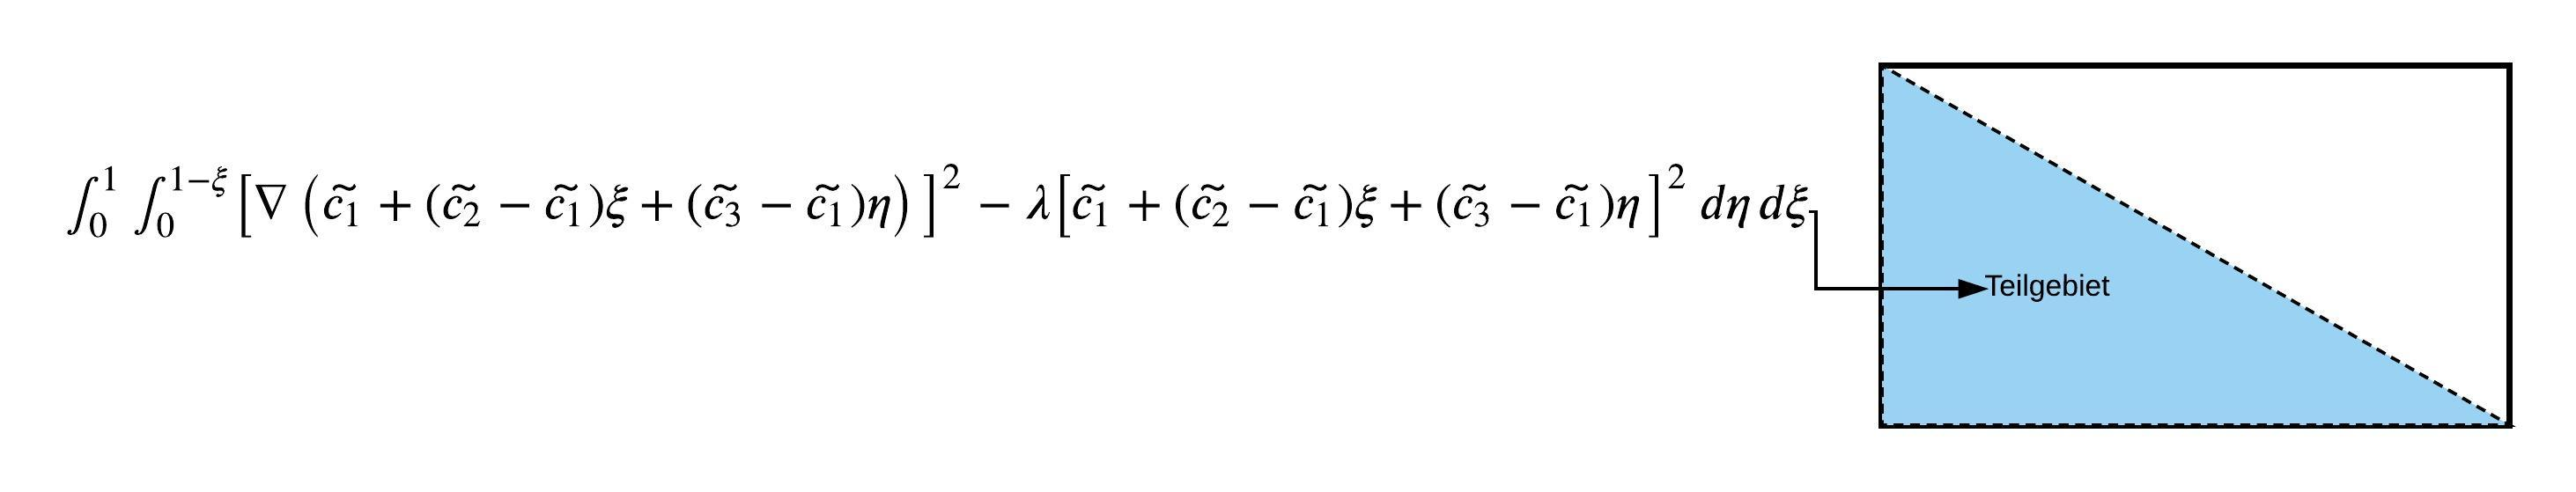
\includegraphics[scale=0.8]{papers/fem/Images/FoTeilgebiet.jpeg}
	\caption{Anwenden des Minimalprinzipes auf jedes Teilgebiet}
	\label{fig:schemNMR_vorlage}
\end{figure}

Nun kann der erste Teil der Berechnung beginnen. Die partielle Ableitung nach dergewählten linearen Funktion $f(u)$ erigbt das Resultat

\begin{equation}
	\nabla u = 	
	\left[ \begin{array}{r}
	c_2  \\
	c_3 \\
	\end{array}\right]
	\label{fem:equationSchwarzquadratischP}
\end{equation} 

Nun ist aber noch die Frage offen wie die Gleichungen zustande kommen für diese Koeffizienten. In folgenden Abschnitt wird dies anhand eines Beispiels beschrieben.

\subsubsection{Gleichungssystem aufstellen 
\label{fem:section:GL}}

Bekannt ist nun wie die Formeln für die einzelne Elemente aussehen. Allerdings stellt sich dann die Frage, wie die das alles in eine Matrix zusammengefasst werden soll, da sich auch quadratische Koeffizienten aus der Ansatzfunktion ergeben $\int_{\Omega u^2 \, dx \, dy}$. Inn der Abbildung \ref{fem:Stuestellen} sind von 2 Dreiecken die Eckpunkt bzw. Stützstellen aufgezeichnet. Es lässt sich erkennen das in 2 Eckpunkten die Stützstellen gleich sind.
\begin{figure}[h]
	\centering
	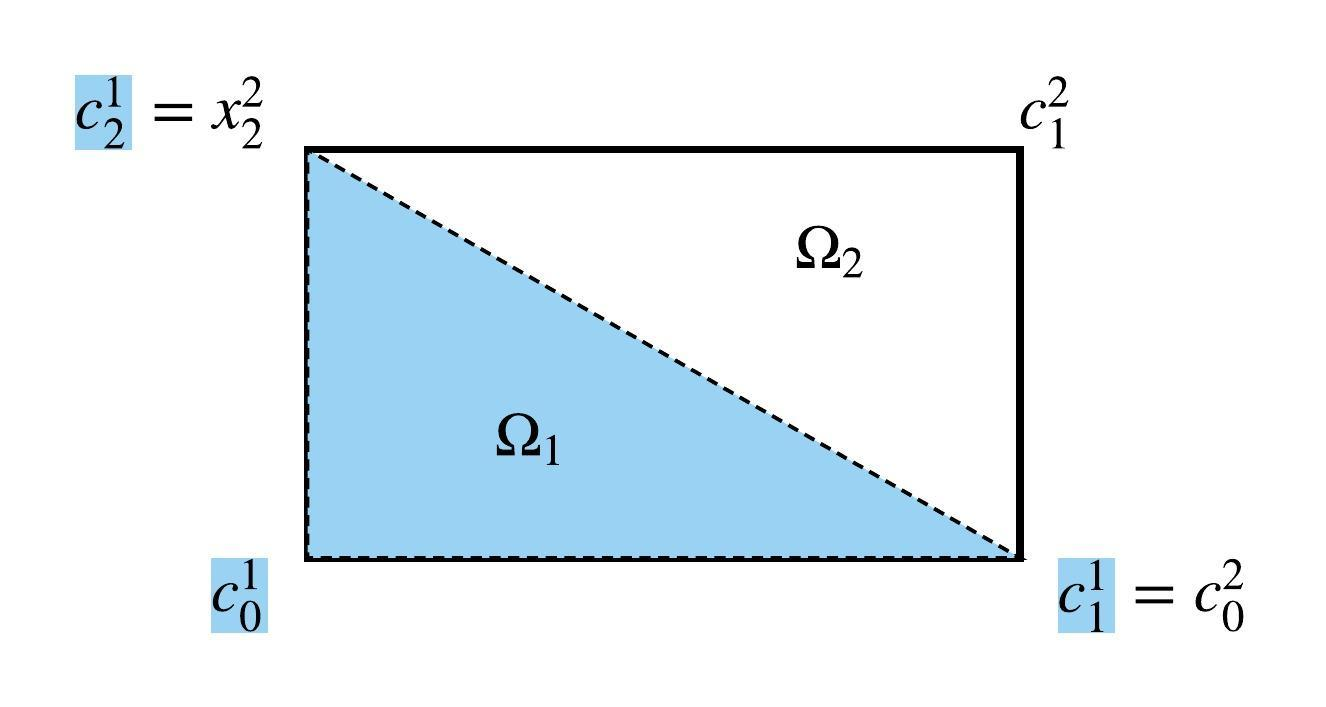
\includegraphics[scale=0.8]{papers/fem/Images/Stuezstellen.jpeg}
	\caption{Stuezstellen der Elemente $\int_{\Omega_1}$ und $\int_{\Omega_2}$ }
	\label{fem:Stuestellen}
\end{figure}

Nach der Formel \eqref{fem:equationSummGebiete} werden die beiden Gebiete aufsummiert zu
\begin{equation}
	\int u = \int_{\Omega_1} u + \int_{\Omega_2} u 
\end{equation}
Der Koeffizienten des Dreiecks $\Omega_i$ kann wie in \eqref{fem:DreiVektor} notiert werden.
\begin{equation}
	\left( \begin{array}{c} c_0^i \\\ c_1^i \\\ c_2^i \\\ \end{array}\right)
	\label{fem:DreiVektor}
\end{equation}
Um nun quadratische Koeffizienten in der Matrixschreibweise zu erhalten wird diese wie folgt Notiert.
\begin{equation}
\begin{bmatrix}
c_0^1 &  c_1^1 &  c_2^i1  
\end{bmatrix}
\begin{bmatrix}
\ddots & \dots &  \dots    \\
\vdots & \ddots &   \\
\vdots &  & \ddots
\end{bmatrix}
\begin{bmatrix}
c_0^1  \\
c_1^1 \\
c_2^1
\end{bmatrix}
+
\begin{bmatrix}
c_0^2 &  c_1^2 &  c_2^2    \\   
\end{bmatrix}
\begin{bmatrix}
\ddots & \dots &  \dots    \\
\vdots & \ddots &   \\
\vdots &  & \ddots
\end{bmatrix}
\begin{bmatrix}
c_0^2  \\
c_1^2 \\
c_2^2
\end{bmatrix}
	\label{fem:MatrixKoeffizient}
\end{equation}
Die ist auch die Begründung für die später verwendete Formel \eqref{fem:Minimal2LinAlg}.
%Für jedes Flächenelement gilt die Gleichung \ref{fem:MinimalproblemElement}. Nun müssen alle diese Elemente in eine Matrix umgeschrieben werden die sich wie folgt zusammensetzen lässt.

\begin{equation}
			\underbrace{ \int_{\Omega} (\nabla u)^2 dx \, dy} \, -  \, \underbrace{\lambda \int_{\Omega} u^2 dx \,dy}
			\label{fem:Minimal2TermLinAlg}
\end{equation}


\begin{equation}
			c^t Ac \, - \, \lambda c^t Bc
			\label{fem:Minimal2LinAlg}
\end{equation}
Die Matrix $A$ wird gebildet durch die Teilmatrizen eines jeden Flächenelements. Die Teilmatrix eines Flächenelements besteht  aus dem Integral des 1. Terms von \ref{fem:Minimal2TermLinAlg} 

\begin{equation}
			\int_0^1 \int_0^{1 - \xi} \left( \begin{array}{c} c_2 \\ c_3\\	
\end{array} \right)^2 d\eta \, dxi
			\label{fem:Minimal2LinAlgA}
\end{equation}
was dann zu der entsrechenden Teilmatrix eines Dreiecks führt

\begin{equation}
	A_{\triangle} = \left( \begin{array}{cc}
	c_2^2 \int_{\Omega} 1 dx \, dy & 0  \\ 
	0 & c_3^2 \int_{\Omega} 1 dx \, dy  \\
	\end{array}\right)
	\label{fem:TeilmatrixA}
\end{equation}
und wird dann in die Matrix $A $eingefügt bzw. zusammengefasst, dass  somti sämtliche Teilmatrizen aller Flächenelemente in der Matrix $A$ vorhanden sind. Eine jede Farbe soll veranschaulichen, dass dies ein Dreieck- Flächenelement darstellt.

\begin{equation}
 A = \begin{pmatrix} 0 & 0 & \hdotsfor{4} & 0 \\
	0 & \textcolor{green}{ c_2^2 \int_{\Omega} 1 dx \, dy }& \vdots & 0 & \vdots & & \vdots \\
	\vdots & \vdots & \textcolor{green}{c_3^2 \int_{\Omega} 1 dx \, dy }& 0 & \vdots  & & \\
	\vdots & \vdots & 0 & \ddots & \textcolor{red}{ c_2^2 \int_{\Omega} 1 dx \, dy }& & \\
	\vdots & \vdots & 0 & 0 & 0 & \textcolor{red}{c_3^2 \int_{\Omega} 1 dx \, dy} & \\
	0 & \hdotsfor{2} & 0 &  & & &  \ddots  \\
	\end{pmatrix}
	\label{fem:MatrixA}
\end{equation}
Etwas anders zusammengefasst dargestellt wie die Matrix $A$ aus den Teilmatrizen $A_{\triangle}$ besteht.

\begin{equation}
 A =	\begin{pmatrix}
	A_{\triangle_1} & 0 & \cdots & \cdots & 0 \\
	0 & \ddots & \vdots & 0 & \vdots \\
	\vdots & \vdots & \ddots & 0 & \vdots \\
	\vdots & \vdots & 0 & A_{\triangle_i} & \vdots \\
	0 & \cdots & \cdots & 0 &  \ddots \\
	\end{pmatrix}
\end{equation}

Die Matrix $A$ ist nun bekannt. Es fehlt jedoch noch die Matrix $B$, um das Gleichungs-System zu komplettieren. Die Matrix $B$ wird nun wie folgt definiert. Um die folgende Form zu erhalten muss lediglich der rechte Term von \ref{fem:Minimal2D2Term} für die einzelne Koeffizienten berechnet werden was dann den folgenden Ausdruck ergibt

\begin{equation}
			\int_0^1 \int_0^{1 - \xi}  \textcolor{cyan}{c_0^2} + \textcolor{blue}{c_1^2 x^2} + \textcolor{red}{c_2^2 y^2} + \textcolor{green}{2 c_0 c_1 x} + \textcolor{orange}{2 c_0 c_2 y} +\textcolor{purple}{ 2 c_1 c_2 xy} \,  d\eta \, d \xi
			\label{fem:Minimal2LinAlgB}
\end{equation}
Nun soll dies wieder in die Matrix- Schreibweise übertragen werden was dann eine Teilmatrix $B$ eines Dreickes entspricht

\begin{equation}
 B_{\triangle} = \left( \begin{array}{ccc}
	\textcolor{cyan}{- \lambda \int_{\Omega} 1} &  \textcolor{green}{- \lambda \int_{\Omega} x} & \textcolor{orange}{- \lambda \int_{\Omega} y}  \\
	\textcolor{green}{- \lambda \int_{\Omega}x} & \textcolor{blue}{- \lambda \int_{\Omega} x^2} &  \textcolor{purple}{- \lambda \int_{\Omega} xy} \\
	\textcolor{orange}{- \lambda \int_{\Omega} y} & \textcolor{purple}{- \lambda \int_{\Omega} xy} & \textcolor{red}{ - \lambda \int_{\Omega} y^2} \\
	\end{array}\right)
	\label{fem:MatrixB}
\end{equation}
Diese Teilmatrix $B$ eines jeden Flächenelements wird dann wieder analog der Matrix $A$ in eine Matrix $B$ eingesetzt, so dass diese dann alle Teilmatrizen aller Dreieck-  Flächenstücke enthält.

\begin{equation}
B =	\begin{pmatrix}
	B_{\triangle_1} & 0 & \cdots & \cdots & 0 \\
	0 & \ddots & \vdots & 0 & \vdots \\
	\vdots & \vdots & \ddots & 0 & \vdots \\
	\vdots & \vdots & 0 & B_{\triangle_i} & \vdots \\
	0 & \cdots & \cdots & 0 &  \ddots \\
	\end{pmatrix}
\end{equation}


\subsection{Schritt 3 Minimalprinizip anwenden auf Approximation}

Nun folgt der nächste Schritt nämlich das Minimieren des quadratischen Ausdrucks
\begin{equation}
	c^t Ac - c^t \lambda Bc
\end{equation}
Was so viel bedeutet wie nach den Koeffizienten $c_k$ ableiten was für den  für 1. Term
\begin{equation}
	\nabla c^t Ac = 2Ac
\end{equation}
ergibt und für den 2. Term den Ausdruck

\begin{equation}
	\nabla c^t \lambda Bc = 2\lambda Bc
\end{equation}
Diese Ableitungen erscheinen nicht gerade ersichtlich insbesondere der Faktor 2. 

Das ableiten im 1- Dimensionalen Raum ergibt nach der klassichen Analysis

\begin{equation}
	\frac{d}{dx} ax^2 = 2ax
\end{equation}
Um die Ableitung in einem n-Dimensionalen, quadratischen Matrix vorzunehmen muss diese erst in einen Summennotation umgeschrieben werden wie folgt

\begin{equation}
			x^tAx, x \in \mathbb{R}^n
\end{equation}
Zu erkennen ist, dass nach der Ableitung von $x$ die Produkt- Regel zum tragen kommt. 

\begin{equation}
	\sum_{i,j} \frac{\partial x_i}{\partial x_n} a_{ij} x_j + \sum_{i,j} x_i a_{ij} \frac{\partial x_j}{\partial x_n}
\end{equation}
Dies kann vereinfacht werden anhand der folgenden Kürzungs- Berechnung:

\begin{equation}
	\sum_{j} a_{nj} x_j + \sum_{i,j} x_i a_{in} = \sum_{j} a_{nj} x_j + \sum_{\textcolor{red}{\not{j}} i} a_{n \textcolor{red}{\not{j}} i} x_{\textcolor{red}{\not{j}} i} = 2(Ax)_n
\end{equation}

\subsection{Schritt 4 Gleichungssystem aufstellen}
Nun kann das Gleichungssystem aufgestellt werden.
\begin{equation}
	2Ac - 2\lambda Bc = 0 \Rightarrow (A-\lambda B)c = 0
	\label{fem:GLLang}
\end{equation}
Durch das umschreiben der Gleichung \ref{fem:GLLang} ist ersichtlich, dass es sich um ein Eigenwertproblem für die Matrix $B^{-1}A$ handelt.

\begin{equation}
		B^{-1}Ac = \lambda c
 \end{equation}
 Dieses kann z.B. durch das Jacobi Verfahren, beschrieben im Kapitel 6.4 gelöst werden.
 
\subsection{Andere lineare Ansatzfunktionen
\label{fem:subsection:Ansatzfunktionen}}

Neben dem durchgerechneten Beispiel des Einheitsdreiecks kann auch eine andere Formfunktion verwendet werden. Die folgende Formfunktion gilt für den linearen Ansatz eines Parallelogramms.

\begin{equation}
	u(x,y) = c_1 + c_2 x + c_3 y + c_4 xy
\end{equation} 


\subsubsection{Quadratischer Ansatz
\label{fem:subsection:bonorum}}

Der Vorteil des quadratischen Ansatzes liegt darin, dass die Freiheitsgeraden erhöht werden. Somit kann unter umständen eine bessere Approximation erreicht werden.
Zu beachten ist allerdings, dass diese die Matrix enorm aufblasen bzw. vergrössern und dann mehr Ressourcen in Anspruch nehmen, um die Matrix bzw. die Eigen werte zu berechnen.

In der Gleichung \ref{fem:equationSchwarzquadratischD}  ist der Ansatz für das Einheitsdreieck gegeben. Und in der Gleichung \ref{fem:equationSchwarzquadratischP} der quadratische Ansatz für ein Einheitsparallelogramm.

\begin{equation}
	u(x,y) = c_1 + c_2 x + c_3 y + c_4 x^2 + c_5 xy + c_6 y^2
	\label{fem:equationSchwarzquadratischD}
\end{equation}

\begin{equation}
	u(x,y) = c_1 + c_2 x + c_3 y + c_4 x^2 + c_5 xy + c_6 y^2 + c_7 x^2y + c_8 xy^2
	\label{fem:equationSchwarzquadratischP}
\end{equation} 



